\documentclass[10pt]{article}
\usepackage[margin=0.7in]{geometry}
\usepackage[T1]{fontenc}
\usepackage{graphicx,hyperref}
\begin{document}
\section*{Nonmonic native polynomial division}
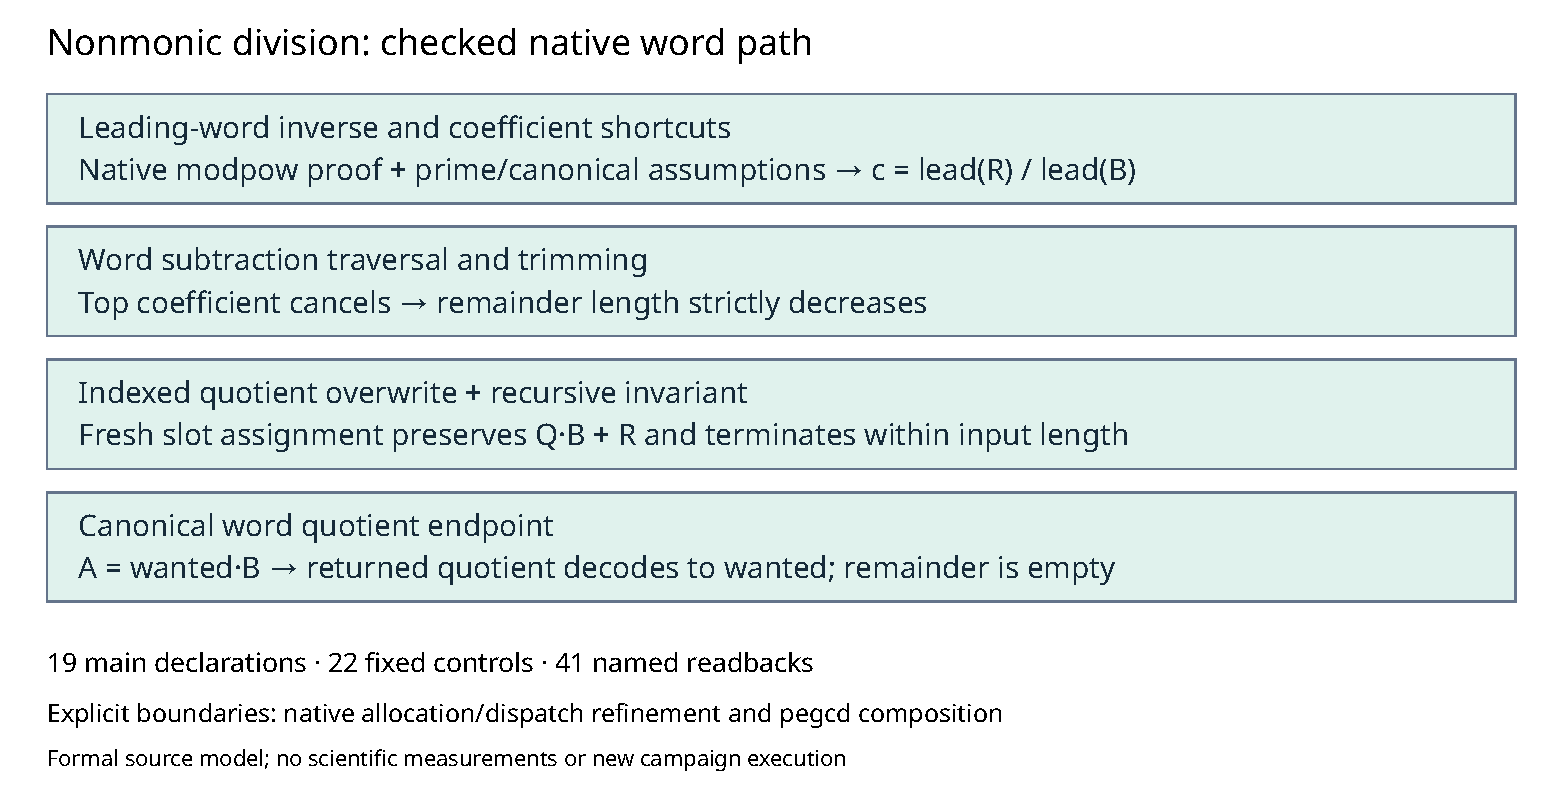
\includegraphics[width=\linewidth]{flow.pdf}

The construction extends native word division from monic divisors to arbitrary canonical nonzero leading words. Nineteen main declarations and twenty-two fixed controls have forty-one named axiom readbacks.

\paragraph{Source and assumptions.}
The bound source is three\_leads.rs, lines195--209,210--226,307--333 and849--880. The native division uses the last divisor word without trimming it. Its inverse shortcut and coefficient shortcut are both modeled. Assumptions are prime modulus, canonical input/divisor words, nonzero last divisor word, and $1<p<2^{31}$. Native correspondence is scoped to odd-prime, degree-one, no-table Field dispatch. Fuel at least the original input length suffices.

\paragraph{Derived inverse and descent.}
The inverse is derived through the existing checked widened modular exponentiation and Fermat proof. The coefficient equals the leading remainder coefficient divided by the leading divisor coefficient. Per-index word subtraction cancels the top coefficient; trimming strictly decreases remainder length.

\paragraph{Exact storage endpoint.}
The quotient loop uses indexed overwrite into a zero-initialized finite UInt64 array of the source slot count. Its refinement proves the invariant $QB+R=A$. For an exact input identity $A=WB$, the actual trimmed output words are canonical, decode to $W$, and have empty remainder. The theorem does not assume that the loop returns $W$.

\newpage
\section*{Checks, controls and boundaries}
\paragraph{Fixed controls.}
Fourteen coefficient/step controls cover inverse2 modulo17, both shortcuts, coefficient6/2=3, zero numerator, two exact steps, nonexact remainder, empty and zero-leading divisors, and composite-modulus inverse failure. Eight full word controls cover exact and nonexact outputs, zero input, padded input, constant divisor, short input, insufficient fuel, and monic agreement.

\paragraph{Native workflow.}
Lean runs through a thin shell wrapper with fresh attempt directories, source/dependency SHA256 bindings, stdout/stderr and native exit propagation. Compiled Rust validates receipts, current source bytes, exact named inventory and allowed axioms. Its six rejection controls cover bad native exit, changed bindings, wrong module, forbidden axiom, missing name and empty inventory. No Python verifier is used.

\paragraph{Retained failures.}
One coefficient proof needed simplification rather than definitional equality for the coerced word1. One generalized-loop call had transposed arguments. Both failed native receipts are retained; corrected modules passed.

\paragraph{Scope.}
The model recomputes the pure inverse expression inside the coefficient function while native code caches it; this proves semantics and makes no operation-count claim. Native allocation byte/isize limits, compiled Rust equivalence, instrumentation and other Field dispatches remain separate. The prior explicit allocation bound applies to the unchanged slot count. Pegcd and Cantor composition remain next interfaces. No scientific runs or cloud operations occurred; the full cohort scope and expired campaign limits remain unchanged.

\paragraph{Evidence.}
See REPORT.md, status.json, acceptance.json, expected-names.txt, and the attempt directories beside this PDF. Source and dependency hashes are retained in each receipt's before.sha256. The existing wide-modpow, monic remainder and quotient-storage packets supply the checked finite-field and polynomial foundations. Publication precedes independent review.
\end{document}
